%Experimental Results and Analysis – in this section, you should show the quantitative results – charts and tables. Analyze the results by explaining and highlighting what is important on them in terms of your goals and what is bad. You should explain the strange results too.

%V ďalšej časti prezentujte vlastný prínos a vlastné výsledky porovnajte s výsledkami iných. Charakterizujte použité metódy.
%Vyhýbajte sa používaniu žargónu.
%Používajte starú múdrosť: 1 obrázok je viac než 1000 slov.

\subsection{Handwritten Digits} 
\label{sec:results-digits} 

In this section we wanted to test TLR on high dimensional graphical task and compare it to other known models. Therefore we have chosen the \emph{hand written digits} dataset (\ref{sec:datasets-digits}). As in the previous simulations, we trained the networks for range of $\lambda_v$ and $\lambda_h$ values and found best parameters. Then we analysed that particular network more closely. 

For this task we splitted the dataset to \emph{train} set with 38,000 samples and \emph{test} set with 4,000 samples. First we trained the networks on the train set and then evaluted them on the test set. Also the convergence criteria were different. The $Epoch_{\rm max}$ value was set to 20 and if no $patSucc^F$ increase occured in the previous 3 epoch, then the training was stopped. Note that the final classification method was chosen from treshold perceptron to classifying the output value with greatest activation. 

%===============================================================
%===============================================================
%===============================================================
\subsubsection{Two learning rates} 
\label{sec:tlr-digits} 
On figure~(\ref{fig:results-tlr-digits-epoch}) $patSucc^F$, i.e. ratio of correctly classified test samples, is plotted for $(\lambda_v,\, \lambda_h)$ pairs. In comparison to TLR performances on tasks 4-2-4 encoder~(\ref{fig:results-tlr-auto4-performance}) and CBVA~(\ref{fig:results-tlr-k3-performance}) the successful values of $(\lambda_v,\, \lambda_h)$ were smaller. That introduces the hypothesis that the bigger set of samples, the lower the values of $(\lambda_v,\, \lambda_h)$. We suggest it as a possible future work in section~\ref{sec:future-work}. 

%Purpose: 
%======== (3D) L1 x L2 x patSuccF =========
%======== (3D) L1 x L2 x epochs =========
\begin{figure}[H]
  \centering
  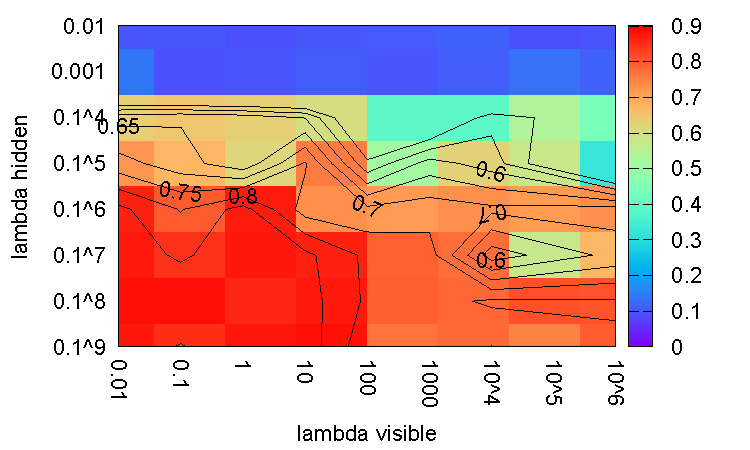
\includegraphics[width=0.60\textwidth]{img/tlr-digits-psf.pdf} 
%  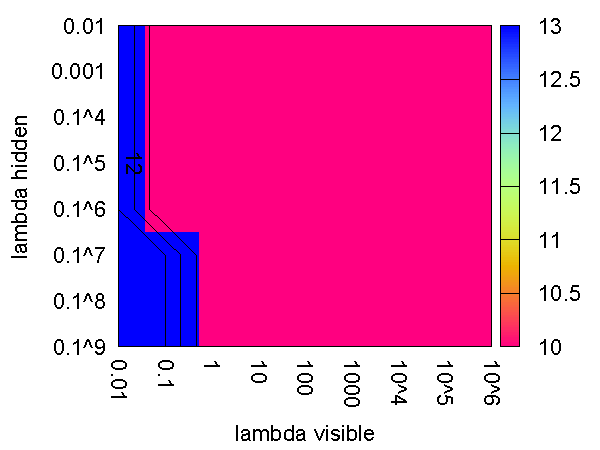
\includegraphics[width=0.49\textwidth]{img/tlr-digits-epoch.pdf}     
  \caption{TLR performance on the \emph{digits} task for $\sigma = 1/\sqrt{784+1} \approx 0.036$ and $\mu = 0.01$ best being $88.47\$$ with $\lambda_v=0.1$ and $\lambda_h=10^{-8}$.}
  \label{fig:results-tlr-digits-success}
\end{figure}

On the following figure~(\ref{fig:results-tlr-digits-epoch}) $patSucc^F$ is plotted to epochs. TODO explain. 

%======== (2D) best TLR on ALL_SUCC x epoch (std-dev) ==========
\begin{figure}[H]
  \centering
  
\includegraphics[width=0.60\textwidth]{img/placeholder.png}  %TODO    
  \caption{TLR success evolution for the \emph{digits} task with $\sigma = 1/\sqrt{784+1}$, $\mu = 0.01$, $\lambda_v=0.1$ and $\lambda_h=10^{-8}$.}
  \label{fig:results-tlr-digits-epoch} 
\end{figure}

%===============================================================
%===============================================================
%===============================================================
\subsubsection{Comparison} 
\label{sec:results-cmp-digits} 

For comparison of TLR on the \emph{digits} task we have chosen from \citet{digits2014mnist} neural network models with similar architecture of layers, i.e. 784-300-10. The table~\ref{tab:results-cmp-digits} shows the comparison where we see that TLR is able to learn such tasks but still has a great performance gap to fill. 

\begin{table}[H] 
  \centering
    \begin{tabular}{|l|l|l|l|l|}
    \hline
    Algorithm (section)&$\lambda_h$&$\lambda_v$&$patSucc^F$ &Epochs\\ %&SEM(success) \\
    \hline
    Linear classifier & -- & -- & 88 & -- \\ %&1.52e+08\\
    \hline
    BP 784-300-10~(\ref{sec:models-bp})& -- & -- & 95.3 & -- \\ %&1.52e+08\\
    \hline 
    TLR 784-300-10~(\ref{sec:models-bp})& $10^{-8}$ & 0.1 & 88.47 & -- \\ %&1.52e+08\\
    \hline 
    \end{tabular}
  \caption{Comparing performance of different models on the \emph{digits} task with 300 hidden neurons. Data from \citet{lecun1998gradient} and \citet{digits2014mnist}.} 
  \label{tab:results-cmp-digits}
\end{table}

%===============================================================
%===============================================================
%===============================================================
\subsubsection{Backward representations} 
\label{sec:our-backward-repre}

The method of \emph{backward representations} for \emph{hetero--associative} tasks, i.e.~tasks which have multiple inputs for the same output, is to \emph{depict} the backward activation of an output. In case of BAL~(\ref{sec:models-bal}), the backward representations are all possible values of $x^{\rm B}$ for each possible output value, i.e.~target. For example the backward representation of digit "8" in TLR~(\ref{sec:our-tlr}) is show on figure~\ref{fig:our-backward-repre-9}. 

\begin{figure}[H]
  \centering
  
\includegraphics[width=0.2\textwidth]{img/tlr-digit-8.png} 
  \caption{Backward representation of digit "8" in TLR.}
  \label{fig:our-backward-repre-8}
\end{figure}

As we can see on figure~\ref{fig:results-tlr-digits-backward}, TLR gives us readable backward activations. This intuitively proves that the model is capable of bidirectional training. The shapes could be best seen on digit ``0'', ``1'' and ``8''. But using a little creativity we could see other shapes too. 

%======== (2D) for best network vs. sample digits
\begin{figure}[H]
%TODO rotate 
  \centering
  
\includegraphics[width=0.98\textwidth]{img/tlr-digits.png}    
  \caption{Backward representations for the most successful TLR instances on the \emph{digits} task.}
  \label{fig:results-tlr-digits-backward} 
\end{figure}
